% =====================================================================
% BMED365-2027: Lab Quick Start — AI-Assisted Python with Productive Friction
% =====================================================================
\documentclass[aspectratio=169, 10pt]{beamer}

\usepackage[utf8]{inputenc}
\usepackage[T1]{fontenc}
\usepackage[english]{babel}
\usepackage{graphicx}
\usepackage{booktabs}
\usepackage{amsmath}
\usepackage{listings}
\usepackage{xcolor}
\usepackage{hyperref}
\hypersetup{
    colorlinks=true,
    linkcolor=blue!70!black,
    urlcolor=blue!70!black,
    citecolor=green!50!black
}

\usetheme{Madrid}
\usecolortheme{beaver}
\setbeamertemplate{navigation symbols}{}

\definecolor{codegreen}{rgb}{0,0.6,0}
\definecolor{codegray}{rgb}{0.5,0.5,0.5}
\definecolor{codepurple}{rgb}{0.58,0,0.82}
\definecolor{backcolour}{rgb}{0.95,0.95,0.92}

\lstdefinestyle{mystyle}{
    backgroundcolor=\color{backcolour},
    commentstyle=\color{codegreen},
    keywordstyle=\color{magenta},
    numberstyle=\tiny\color{codegray},
    stringstyle=\color{codepurple},
    basicstyle=\ttfamily\scriptsize,
    breakatwhitespace=false,
    breaklines=true,
    captionpos=b,
    keepspaces=true,
    numbers=left,
    numbersep=5pt,
    showspaces=false,
    showstringspaces=false,
    showtabs=false,
    tabsize=2
}
\lstset{style=mystyle}

\title[Quick Start: AI \& Python]{Lab Quick Start: AI-Assisted Python Programming}
\subtitle{Learning with Productive Friction in Computational Imaging, Modeling \& Biomedical AI}
\author[A. Lundervold (BMED365)]{Arvid Lundervold}
\institute[UiB \& MMIV]{Department of Biomedicine \& MMIV, University of Bergen\\BMED365 --- Spring 2027}
\date{Tuesday 12 January 2027 $\cdot$ 09:15--13:00}

\begin{document}

% ---------------------------------------------------------------------
\begin{frame}
    \titlepage
\end{frame}

% ---------------------------------------------------------------------
\begin{frame}{Session Overview}
    \tableofcontents
\end{frame}

% =====================================================================
\section{BMED365 \& AI-Assisted Learning with Friction}
% =====================================================================

\begin{frame}{Welcome to BMED365 (Spring 2027)}
    \begin{columns}[T,onlytextwidth]
        \column{0.48\textwidth}
        \textbf{Core Course Aims:}
        \begin{itemize}
            \item Build practical \textbf{computational thinking} for biomedicine and precision healthcare.
            \item Combine \textbf{machine learning}, \textbf{network science}, \textbf{deep learning}, and \textbf{generative AI} with clinical rigor.
            \item Connect \textbf{3D medical imaging} with \textbf{mechanistic modeling} \& Digital Twins.
            \item Practice \textbf{explainable, ethical, and verifiable AI} (EU AI Act, open science).
        \end{itemize}

        \column{0.50\textwidth}
        \textbf{Two-Block Course Arc:}
        {\footnotesize
        \begin{itemize}
            \item \textbf{Block 1 (January):}
            \begin{itemize}\footnotesize
                \item \textbf{Lab 0:} Tabular ML \& AutoML (\texttt{PyCaret})
                \item \textbf{Lab 1:} Patient Similarity Networks (\texttt{NetworkX})
                \item \textbf{Quick Start:} Python + AI with friction \textit{(today!)}
                \item \textbf{Lab 2:} Deep Learning (CNNs, ECG/MRI, Grad-CAM)
                \item \textbf{Lab 3:} GenAI, LLMs, XAI \& Neurosymbolic AI
                \item \textbf{Team Project:} Glioblastoma precision medicine
            \end{itemize}
            \item \textbf{Block 2 (February):}
            \begin{itemize}\footnotesize
                \item \textbf{Lab 4:} Comp.\ Imaging \& \textbf{Kiwi 7\,T MRI}
                \item \textbf{Lab 5:} Comp.\ Modeling \& \textbf{Kiwi Digital Twin}
                \item \textbf{Individual Project:} Speed poster presentation
            \end{itemize}
        \end{itemize}
        }
    \end{columns}
\end{frame}

% ---------------------------------------------------------------------
\begin{frame}{Why Learn Python in 2027 When AI Can Write Code?}
    \begin{columns}[T,onlytextwidth]
        \column{0.52\textwidth}
        \textbf{Empirical Evidence: AI Tutor vs.\ AI Crutch}
        \begin{itemize}
            \item \textbf{Unrestricted AI hurts retention:} Unguarded ChatGPT boosted practice scores (+48\%) but \textbf{lowered subsequent unassisted exam scores by 17\%}, whereas a Socratic AI tutor preserved learning (\href{https://doi.org/10.1073/pnas.2422633122}{Bastani et al., \textit{PNAS} 2025}).
            \item \textbf{Scaffolded tutoring excels:} A Harvard RCT showed a hint-based AI tutor \textbf{more than doubled learning gains} over active-learning lectures (\href{https://doi.org/10.1038/s41598-025-97652-6}{Kestin et al., \textit{Sci.\ Rep.} 2025}).
            \item \textbf{Clinical stakes:} Routine AI reliance risks clinician \textit{deskilling} (\href{https://doi.org/10.1016/S2468-1253(25)00133-5}{Budzy\'n et al., \textit{Lancet Gastroenterol.} 2025}) and trainee \textbf{\textit{never-skilling}} (\href{https://doi.org/10.1038/s41591-026-04438-y}{Ke et al., \textit{Nature Medicine} 2026}).
        \end{itemize}

        \column{0.45\textwidth}
        \begin{block}{Insights from \href{https://co-existence.ai/}{\textit{Co-Existence}} (Mollick, 2026)}
            \footnotesize
            \begin{enumerate}
                \item \textbf{Jagged Frontier:} Models write clean code yet fail silently on units, leakage, or 2D/3D MRI geometry.
                \item \textbf{Centaur \& Cyborg $>$ Blind Conjurer:} Stay in the loop; avoid becoming a \textit{``reverse centaur''}.
                \item \textbf{Human Edge:} Deep \& wide knowledge, \textit{taste} (scientific judgment), and \textit{agency}.
                \item \textbf{Reality Checks AI:} Executable code + physical units test claims immediately!
            \end{enumerate}
        \end{block}
    \end{columns}
\end{frame}

% ---------------------------------------------------------------------
\begin{frame}{Our Quick Start Rule: Productive Friction}
    \footnotesize
    Following \href{https://bjorklab.psych.ucla.edu/wp-content/uploads/sites/13/2016/04/EBjork_RBjork_2011.pdf}{Bjork \& Bjork's \textit{desirable difficulties}}, every module today builds in \textbf{deliberate cognitive friction}:
    \vspace{0.2cm}

    \begin{table}
        \centering
        \begin{tabular}{@{}p{0.24\textwidth}p{0.34\textwidth}p{0.36\textwidth}@{}}
            \toprule
            \textbf{Friction Habit} & \textbf{Passive Crutch (Avoid)} & \textbf{Active Practice (Today)} \\
            \midrule
            \textbf{1. Predict First} & Pressing \texttt{Shift+Enter} blindly & Guess what \texttt{"120" + "80"} or \texttt{list[1]} outputs \textit{before} running \\
            \textbf{2. Attempt, Then Hint} & Pasting the exercise straight into AI & Write a 2-min draft; use graduated \texttt{<details>} hints \& Socratic prompts \\
            \textbf{3. Audit Silent Bugs} & Trusting code because it has no syntax error & Catch \texttt{168 cm} vs.\ \texttt{1.68 m}, \texttt{> 38.0} vs.\ \texttt{>= 38.0}, and \texttt{0.0\,$^\circ$C} dropouts \\
            \textbf{4. Reality-Check Data} & Accepting a fluent LLM answer or \texttt{acc=1.0} & Verify unseen test sets, probabilities, \texttt{mm$^3$} voxel units, \& MRI overlays \\
            \bottomrule
        \end{tabular}
    \end{table}
\end{frame}

% =====================================================================
\section{Python \& Jupyter Environments}
% =====================================================================

\begin{frame}{Why Python for Biomedicine?}
    \begin{columns}[T,onlytextwidth]
        \column{0.58\textwidth}
        Python is the shared language of biomedical data science, imaging, and AI:
        \begin{itemize}
            \item \textbf{Readable syntax:} Reads like structured clinical/scientific English (\textit{``executable pseudocode''}).
            \item \textbf{Unmatched biomedical ecosystem:} \texttt{NumPy}, \texttt{Pandas}, \texttt{scikit-learn}, \texttt{NetworkX}, \texttt{PyTorch}, \texttt{NiBabel}, \texttt{MONAI}.
            \item \textbf{Open science:} Free, cross-platform, and reproducible — unlike proprietary black boxes.
        \end{itemize}

        \vspace{0.15cm}
        {\scriptsize
        \begin{tabular}{@{}lp{0.34\textwidth}p{0.42\textwidth}@{}}
            \toprule
            \textbf{Lang.} & \textbf{Strength} & \textbf{Limitation in BMED365} \\ \midrule
            \textbf{Python} & ML/DL, 3D MRI, ODE/PDEs & Raw loops (solved via \texttt{NumPy}) \\
            \textbf{R} & Biostatistics \& omics & Smaller DL / 3D vision stack \\
            \textbf{MATLAB} & Signal \& control eng. & Proprietary license \\ \bottomrule
        \end{tabular}
        }

        \column{0.38\textwidth}
        \centering
        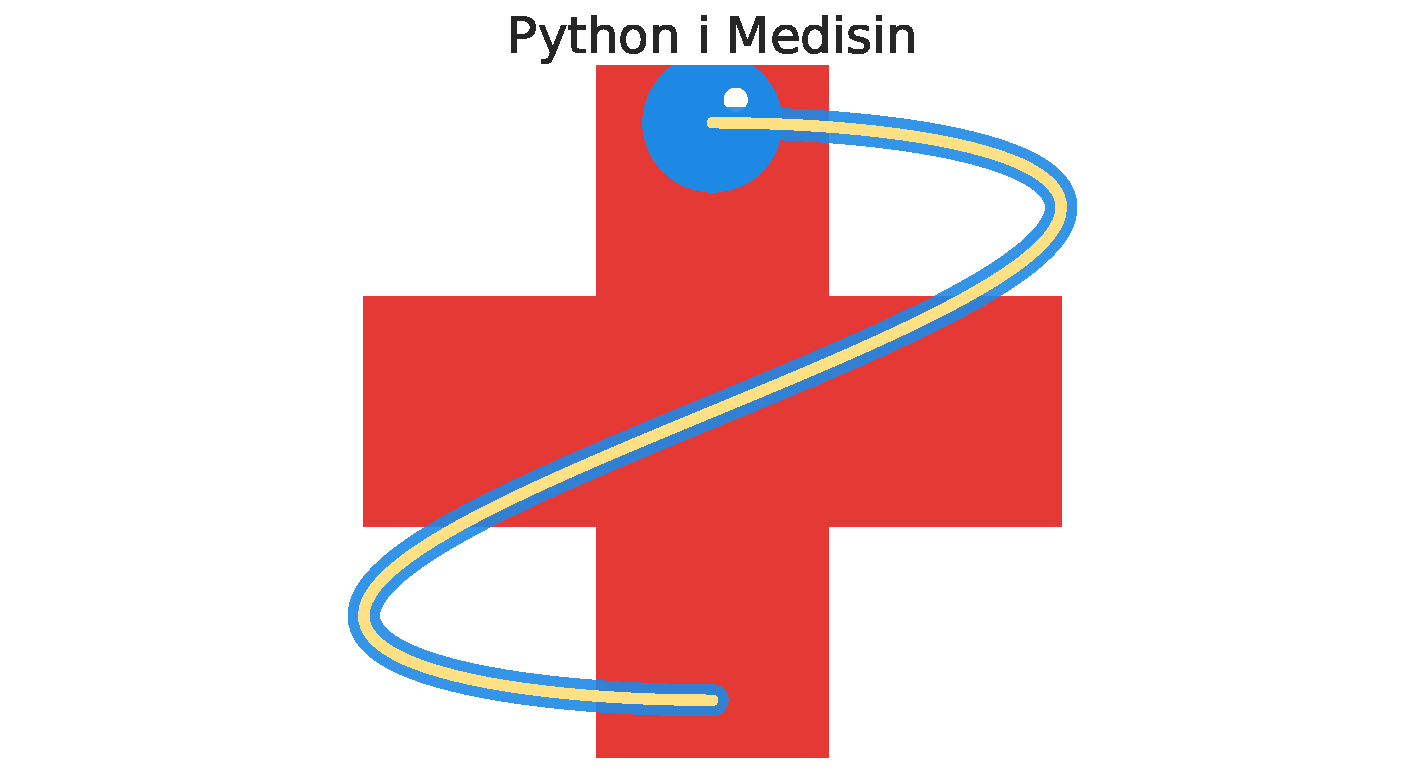
\includegraphics[width=0.68\textwidth]{images/python_medisin.pdf}
        \vspace{0.15cm}

        \begin{block}{\scriptsize AI Transparency}
            \scriptsize You don't need to memorize every library flag --- you need to \textbf{read, test, and judge} what the code computes.
        \end{block}
    \end{columns}
\end{frame}

% ---------------------------------------------------------------------
\begin{frame}[fragile]{Two Seamless Ways to Run \href{https://jupyter.org/}{Jupyter Notebooks}}
    \begin{columns}[T,onlytextwidth]
        \column{0.55\textwidth}
        A \texttt{.ipynb} notebook unites \textbf{Markdown/LaTeX text}, \textbf{executable Python cells}, and \textbf{diagnostic plots} in one reproducible document:
        \begin{itemize}
            \item \textbf{Option 1 --- \href{https://colab.research.google.com/}{Google Colab} (Cloud):} Zero install, runs in any browser, built-in Gemini (\texttt{$\star$}) \& free T4 GPU. \textit{Tip: File $\rightarrow$ Save a copy in Drive!}
            \item \textbf{Option 2 --- Local \texttt{uv} (\texttt{bmed365-2027}):} Pinned Python 3.12 environment (\texttt{pyproject.toml} + \texttt{uv.lock}) in JupyterLab, VS Code, or Cursor.
        \end{itemize}

        \vspace{0.1cm}
        {\footnotesize \textbf{LaTeX math in Markdown:} \verb|$\text{BMI} = w / h^2$| $\longrightarrow$ $\text{BMI} = w / h^2$, and $\text{MAP} = \text{DBP} + \frac{1}{3}(\text{SBP}-\text{DBP})$.}

        \column{0.41\textwidth}
        \centering
        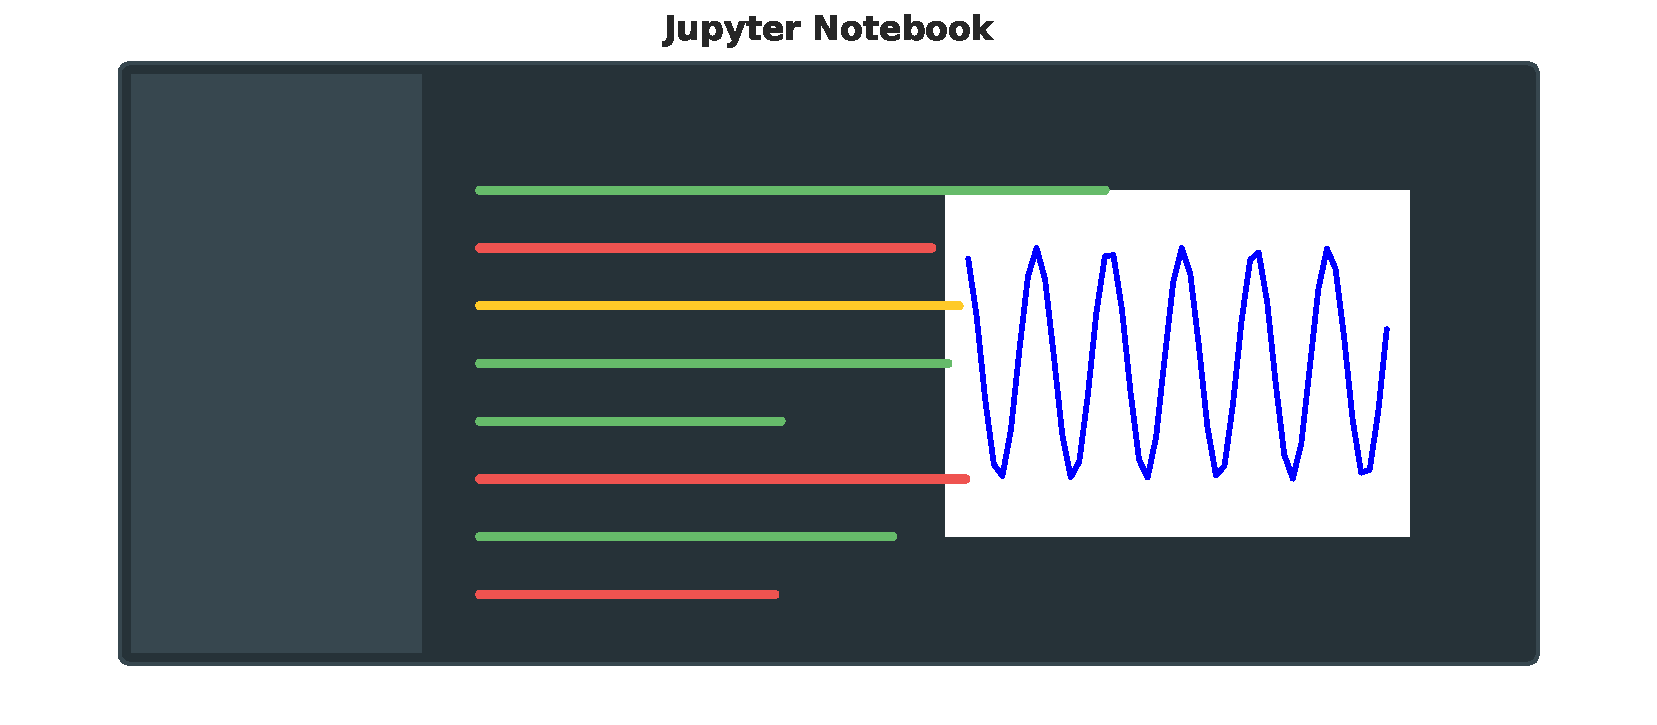
\includegraphics[width=0.66\textwidth]{images/coding_interface.pdf}
        \vspace{0.1cm}

        \begin{alertblock}{\scriptsize Privacy Reminder}
            \scriptsize Course datasets are open-access. \textbf{Never} paste real patient data into consumer AI; use \href{https://chat.uib.no}{chat.uib.no} for UiB work.
        \end{alertblock}
    \end{columns}
\end{frame}

% =====================================================================
\section{Core Scientific Stack \& Clinical Pitfalls}
% =====================================================================

\begin{frame}[fragile]{Python Building Blocks --- and Silent Clinical Bugs!}
    \begin{columns}[T,onlytextwidth]
        \column{0.49\textwidth}
        \textbf{Six building blocks in Modules 2--3:}
        \begin{enumerate}
            \item \textbf{Variables with units:} \texttt{weight\_kg = 72.5}
            \item \textbf{Types:} \texttt{str}, \texttt{int}, \texttt{float}, \texttt{bool}
            \item \textbf{0-indexed lists:} \texttt{bp[0]} is first, \texttt{bp[-1]} is last
            \item \textbf{Decisions:} \texttt{if / elif / else}
            \item \textbf{Loops:} \texttt{for x in readings:}
            \item \textbf{Functions:} \texttt{def screen(temps\_c):}
        \end{enumerate}

        \column{0.48\textwidth}
        \begin{lstlisting}[language=Python]
# AI-generated draft: spots 2 silent bugs?
def ai_fever_screen(temps_c):
    mean_t = sum(temps_c) / len(temps_c)
    has_fever = max(temps_c) > 38.0
    return round(mean_t, 2), has_fever

# Bug 1: 38.0 C returns False (> vs >=)!
# Bug 2: Sensor dropout 0.0 C ruins mean!
        \end{lstlisting}
        \begin{alertblock}{\scriptsize Key Takeaway}
            \scriptsize Code without a \texttt{SyntaxError} can still fail clinically. Always test \textbf{boundary values} and \textbf{sensor dropouts}!
        \end{alertblock}
    \end{columns}
\end{frame}

% ---------------------------------------------------------------------
\begin{frame}{Scientific Libraries Across BMED365}
    \begin{columns}[T,onlytextwidth]
        \column{0.48\textwidth}
        \begin{block}{\href{https://numpy.org/}{NumPy} \& \href{https://matplotlib.org/}{Matplotlib} (Imaging \& Math)}
            \footnotesize
            \begin{itemize}
                \item N-dimensional arrays (\texttt{ndarray}): a 2D MRI slice is a $256\times 256$ matrix; a 3D volume is $256\times 256\times 128$.
                \item Vectorized math \& visual overlays replace guesswork.
            \end{itemize}
        \end{block}

        \begin{block}{\href{https://pandas.pydata.org/}{Pandas} \& \href{https://scikit-learn.org/}{scikit-learn} (Lab 0 ML)}
            \footnotesize
            \begin{itemize}
                \item Tabular patient/biomarker \texttt{DataFrame}s.
                \item \texttt{train\_test\_split}, \texttt{DecisionTreeClassifier}, and \texttt{predict\_proba} for borderline uncertainty.
            \end{itemize}
        \end{block}

        \column{0.48\textwidth}
        \begin{block}{\href{https://networkx.org/}{NetworkX} (Lab 1 PSN)}
            \footnotesize
            \begin{itemize}
                \item Patients as \textbf{nodes}, pairwise similarity as \textbf{weighted edges}.
                \item Degree centrality vs.\ weighted connection strength.
            \end{itemize}
        \end{block}

        \begin{exampleblock}{\footnotesize Socratic AI Prompt Rule}
            \footnotesize
            \textit{``Act as a Socratic Python tutor. Do NOT give me the full solution first --- ask me to predict the output, give one hint at a time, and ask one unit/edge-case check at the end.''}
        \end{exampleblock}
    \end{columns}
\end{frame}

% =====================================================================
\section{Bridge to Block 2: The Kiwi 7T MRI Challenge}
% =====================================================================

\begin{frame}{Module 6 Preview: Pixels, Voxels \& Biophysical Models (Labs 4 \& 5)}
    \begin{columns}[T,onlytextwidth]
        \column{0.43\textwidth}
        \centering
        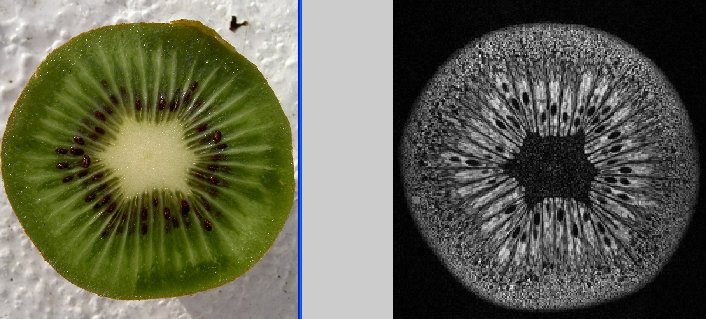
\includegraphics[width=\textwidth,height=0.56\textheight,keepaspectratio]{../../Lab4-Comp-Imag/Kiwi-challenge/assets/photo_mri_kiwi_20050219.jpg}
        \vspace{0.08cm}

        {\scriptsize UiB \textbf{7\,T Bruker Pharmascan} MRI (\texttt{kiwi\_064.png})\\
        16-bit \texttt{uint16} $\cdot$ $0.234 \times 0.234 \times 0.500\text{ mm}^3$}

        \column{0.54\textwidth}
        \footnotesize
        Today's Module 6 connects Python basics directly to our course-wide \textbf{Kiwi 7\,T MRI Challenge}:
        \begin{enumerate}
            \item \textbf{Images are 2D \texttt{NumPy} matrices:} Inspect 16-bit MRI intensities (\texttt{71}--\texttt{32,766}) on equatorial slice $z=64$.
            \item \textbf{Why naive thresholding \& LLM counting fail:} In $T_2$ MRI, the optically white central \textit{columella} turns \textbf{dark} --- merging with seeds! Vision chatbots hallucinate 2D counts and ignore 128-slice 3D geometry.
            \item \textbf{Lab 4 $\leftrightarrow$ Lab 5 Digital Twin bridge:} Compute physical voxel volume ($0.0275\text{ mm}^3$, ``lesion load'') and test Lab 5's 1-line hormone receptor-saturation law:
            \[
                V(N) = V_{\text{basal}} + V_{\max}\frac{N}{K_N + N}
            \]
            predicting $86.1\text{ cm}^3$ at $\hat{N}\approx 1{,}440$ seeds vs.\ measured $85.97\text{ cm}^3$!
        \end{enumerate}
    \end{columns}
\end{frame}

% =====================================================================
\section{Today's Interactive Walkthrough}
% =====================================================================

\begin{frame}{Agenda Inside \texttt{quickstart-ai-python.ipynb} (09:15--13:00)}
    \footnotesize
    \begin{table}
        \centering
        \begin{tabular}{@{}llp{0.56\textwidth}@{}}
            \toprule
            \textbf{Time} & \textbf{Module} & \textbf{Hands-On Activity \& Friction Check} \\
            \midrule
            09:15--09:45 & \textbf{1. Welcome \& Setup} & Colab / local \texttt{uv}, \texttt{print()}, \textit{Predict First:} \texttt{120+80} vs.\ \texttt{"120"+"80"} \\
            09:45--10:30 & \textbf{2. Python Basics} & Variables, BMI \& MAP formulas, \texttt{0}-indexed lists, \texttt{if/for/def} \\
            10:30--10:45 & \textit{Break} & Coffee \& stretch \\
            10:45--11:25 & \textbf{3. AI with Friction} & Centaur/Cyborg modes, tracebacks, \textbf{auditing 2 silent bugs} in \texttt{ai\_fever\_screen} \\
            11:25--12:05 & \textbf{4. ML Taste (Lab 0)} & \texttt{Pandas}, scatter plot, \texttt{DecisionTreeClassifier}, holdout test \& \texttt{predict\_proba} \\
            12:05--12:30 & \textbf{5. Networks (Lab 1)} & \texttt{NetworkX} Patient Similarity Network, centrality \& edge thresholding \\
            12:30--12:50 & \textbf{6. Kiwi 7\,T Bridge} & 16-bit MRI slice array, threshold trap, $\text{mm}^3$ voxels \& $E_{\max}$ growth curve \\
            12:50--13:00 & \textbf{7. Summary} & 60-second unassisted retrieval quiz \& BMED365 roadmap \\
            \bottomrule
        \end{tabular}
    \end{table}
\end{frame}

% ---------------------------------------------------------------------
\begin{frame}{Practical Tips \& The Road Ahead}
    \begin{columns}[T,onlytextwidth]
        \column{0.52\textwidth}
        \textbf{Tips while working in the notebook:}
        \begin{itemize}
            \item \textbf{Run cells top-to-bottom} (\texttt{Shift+Enter}) so variables exist before use.
            \item \textbf{Pause at every \textit{Predict First} \& \textit{Your Turn}} before opening \texttt{<details>} hints.
            \item \textbf{Experiment boldly:} Break a line on purpose, read the last line of the traceback, and fix it.
            \item \textbf{Stuck kernel?} Use \textit{Runtime / Kernel $\rightarrow$ Restart} and run from the top.
        \end{itemize}

        \column{0.44\textwidth}
        \begin{exampleblock}{Next Stops in BMED365}
            \begin{itemize}
                \item \textbf{Fri 15 Jan:} Lab 2 --- Deep Learning
                \item \textbf{Tue 19 Jan:} Lab 3 --- GenAI \& LLMs + Team Project coaching
                \item \textbf{Feb (Block 2):} Lab 4 (Computational Imaging), Lab 5 (Computational Modeling), \& Individual Speed Poster!
            \end{itemize}
        \end{exampleblock}

        \vspace{0.25cm}
        \centering
        \textbf{Let's open \texttt{quickstart-ai-python.ipynb} and begin!}
    \end{columns}
\end{frame}

\end{document}
